\documentclass[tikz,border=10pt]{standalone}
\usepackage{amsmath,amssymb}
\usetikzlibrary{positioning,arrows.meta,shapes.geometric,calc}

\begin{document}
% (GS / DIF-style butterfly: sum on top, difference multiplied by inverse twiddle)
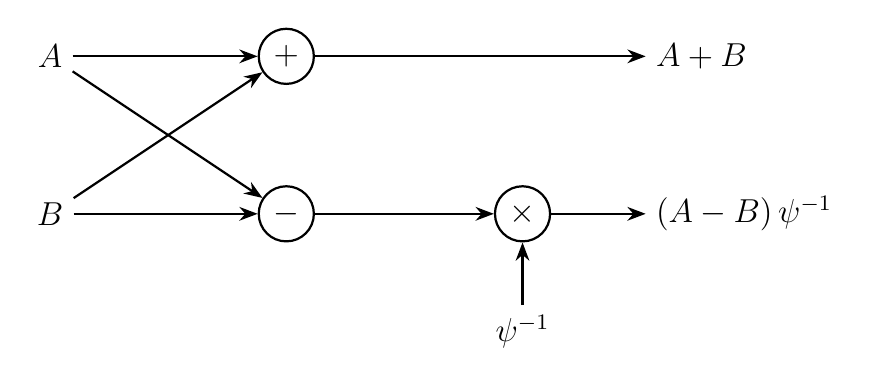
\begin{tikzpicture}[
  >=Stealth,
  node distance=2cm,
  thick,
  op/.style={circle, draw, minimum size=0.7cm, inner sep=0pt, font=\large},
  label_txt/.style={font=\large}
]

% --- Entradas ---
\node[label_txt] (a) at (0,2) {$A$};
\node[label_txt] (b) at (0,0) {$B$};

% --- Operadores (+ e -) ---
\node[op] (plus)  at (3,2) {$+$};
\node[op] (minus) at (3,0) {$-$};

% --- Conexões para (+) ---
\draw[->] (a) -- (plus);
\draw[->] (b) -- (plus);

% --- Conexões para (-) ---
\draw[->] (a) -- (minus);
\draw[->] (b) -- (minus);

% --- Multiplicação no ramo inferior ---
\node[op] (times) at (6,0) {$\times$};
\draw[->] (minus) -- (times);

% --- Fator de rotação inverso (twiddle) ---
\node[label_txt] (psi) at (6,-1.5) {$\psi^{-1}$};
\draw[->] (psi) -- (times);

% --- Saídas ---
\node[label_txt, right=4.2cm of plus]  (out_top) {$A + B$};
\node[label_txt, right=1.2cm of times] (out_bot) {$(A - B)\,\psi^{-1}$};

\draw[->] (plus)  -- (out_top);
\draw[->] (times) -- (out_bot);

% Nota opcional:
% \node[font=\footnotesize, below=0.6cm of out_bot, align=center]
% {Nota: o fator de escala global ($1/2$ ou $1/N$) costuma ser aplicado ao final.};

\end{tikzpicture}
\end{document}
